\PassOptionsToPackage{unicode=true}{hyperref} % options for packages loaded elsewhere
\PassOptionsToPackage{hyphens}{url}
%
\documentclass[]{article}
%
\usepackage{graphicx}
\usepackage{subcaption}
\usepackage{hyperref}

%
\usepackage{lmodern}
\usepackage{amssymb,amsmath}
\usepackage{ifxetex,ifluatex}
\usepackage{fixltx2e} % provides \textsubscript
\ifnum 0\ifxetex 1\fi\ifluatex 1\fi=0 % if pdftex
  \usepackage[T1]{fontenc}
  \usepackage[utf8]{inputenc}
  \usepackage{textcomp} % provides euro and other symbols
\else % if luatex or xelatex
  \usepackage{unicode-math}
  \defaultfontfeatures{Ligatures=TeX,Scale=MatchLowercase}
\fi
% use upquote if available, for straight quotes in verbatim environments
\IfFileExists{upquote.sty}{\usepackage{upquote}}{}
% use microtype if available
\IfFileExists{microtype.sty}{%
\usepackage[]{microtype}
\UseMicrotypeSet[protrusion]{basicmath} % disable protrusion for tt fonts
}{}
\IfFileExists{parskip.sty}{%
\usepackage{parskip}
}{% else
\setlength{\parindent}{0pt}
\setlength{\parskip}{6pt plus 2pt minus 1pt}
}
\usepackage{hyperref}
\hypersetup{
            pdftitle={Assignment 3- cloud computing},
            pdfauthor={Sarit Khirirat},
            pdfborder={0 0 0},
            breaklinks=true}
\urlstyle{same}  % don't use monospace font for urls
\usepackage{longtable,booktabs}
% Fix footnotes in tables (requires footnote package)
\IfFileExists{footnote.sty}{\usepackage{footnote}\makesavenoteenv{longtable}}{}
\usepackage{graphicx,grffile}
\makeatletter
\def\maxwidth{\ifdim\Gin@nat@width>\linewidth\linewidth\else\Gin@nat@width\fi}
\def\maxheight{\ifdim\Gin@nat@height>\textheight\textheight\else\Gin@nat@height\fi}
\makeatother
% Scale images if necessary, so that they will not overflow the page
% margins by default, and it is still possible to overwrite the defaults
% using explicit options in \includegraphics[width, height, ...]{}
\setkeys{Gin}{width=\maxwidth,height=\maxheight,keepaspectratio}
\setlength{\emergencystretch}{3em}  % prevent overfull lines
\providecommand{\tightlist}{%
  \setlength{\itemsep}{0pt}\setlength{\parskip}{0pt}}
\setcounter{secnumdepth}{0}
% Redefines (sub)paragraphs to behave more like sections
\ifx\paragraph\undefined\else
\let\oldparagraph\paragraph
\renewcommand{\paragraph}[1]{\oldparagraph{#1}\mbox{}}
\fi
\ifx\subparagraph\undefined\else
\let\oldsubparagraph\subparagraph
\renewcommand{\subparagraph}[1]{\oldsubparagraph{#1}\mbox{}}
\fi

% set default figure placement to htbp
\makeatletter
\def\fps@figure{htbp}
\makeatother


\title{Assignment 3- cloud computing}
\author{Sarit Khirirat}
%\date{}

\begin{document}
\maketitle

\hypertarget{assignment3spark-on-gcp}{%
\section{Assignment3--Spark-on-gcp}\label{assignment3spark-on-gcp}}

This report is to test the computations of SVD and PCA on the matrix
evaluated by pyspark on google cloud.

\textbf{set-up.} Throughtout this report, the dense square matrices are
randomly generated by normal distribution with zero mean and unit
variance. In addition, we use \texttt{RowMatrix} to distributed the
matrix partitions among the machines within the cluster. Then, we use
SVD and PCA computations available in \texttt{pyspark} to evaluate their
performance among two different clusters.

\hypertarget{requirements}{%
\subsection{Requirements}\label{requirements}}

This section introduces the requirements so that pyspark can be run on
your personal local machine as shown below:

\begin{itemize}
\tightlist
\item
  Java JDK
\item
  Scala
\item
  Spark 2.3.3 with Hadoop 2.7
\item
  Anaconda 3 with the following installed package \texttt{numpy}
\end{itemize}

In addition, you have to export SPARK\_HOME (for your current spark
directory), PYSPARK\_PYTHON (for your current python directory), and
HADOOP\_HOME (for your current hadoop directory) to be able to run the
python scipt on spark.

\hypertarget{run-the-code-in-the-personal-windows-machine}{%
\subsection{Run the code in the personal Windows
machine}\label{run-the-code-in-the-personal-windows-machine}}

After all the installations, we can run the SVD and PCA computations by
the python scipt \texttt{Spark-test-svd-and-pca.py} on your personal
machine with spark 2.3.3 and hadoop 2.7 by using the following command:

\texttt{directory/to/spark-2.3.3-bin-hadoop2.7/bin/spark-submit\ Spark-test-svd-and-pca.py}

\hypertarget{run-the-code-on-gcp}{%
\subsection{Run the code on GCP}\label{run-the-code-on-gcp}}

This section introduces how to test the SVD and PCA computations by the
script \texttt{Spark-test-svd-and-pca.py} on GCP. We follow the detailed
steps which can be found in
\href{https://towardsdatascience.com/step-by-step-tutorial-pyspark-sentiment-analysis-on-google-dataproc-fef9bef46468}{the
following site}.

To be able to run the python scripts on top of spark in the google cloud
platform, we need to

\begin{enumerate}
\def\labelenumi{\arabic{enumi}.}
\item
  Enable Cloud Dataproc API which can be found in the API library in
  your console.
\item
  Create the Bucket which can be found in Web Console. Here, you upload
  necessary python scipts and data matrices.
\item
  Create the clusters to make the numerical evaluations using Dataproc.
  Here, you can easily deploy the clusters which are already installed
  spark and python.
\item
  You can submit the job into the cluster easily from your console.
\end{enumerate}

\hypertarget{numerical-results-for-gcp}{%
\subsection{Numerical Results for GCP}\label{numerical-results-for-gcp}}

We randomly generated the dense matrix with dimension
\(2000\times2000\), \(2100\times 2100\), and \(2200\times 2200\) to
evaluate the performance of distributed computations of SVD and PCA when
we use two different types of clusters: one consists of one master and
another consists of one master and two workers. Throughout the
simulations, we set 2 virtual CPUs and 500 GB memory storage for a
master and each worker.

\begin{longtable}[]{@{}lcr@{}}
\toprule
Cluster type & Matrix Dimension & Running Time\tabularnewline
\midrule
\endhead
1 M 0 W & \(2000\times2000\) & 2 min 22 sec\tabularnewline
& \(2100\times2100\) & 8 min 32 sec\tabularnewline
& \(2200\times2200\) & out of memory\tabularnewline
1 M 2 W & \(2000\times2000\) & 1 min 45 sec\tabularnewline
& \(2100\times2100\) & 1 min 54 sec\tabularnewline
& \(2200\times2200\) & 2 min 0 sec\tabularnewline
\bottomrule
\label{tab:table_1}
\end{longtable}

\begin{figure}
\centering
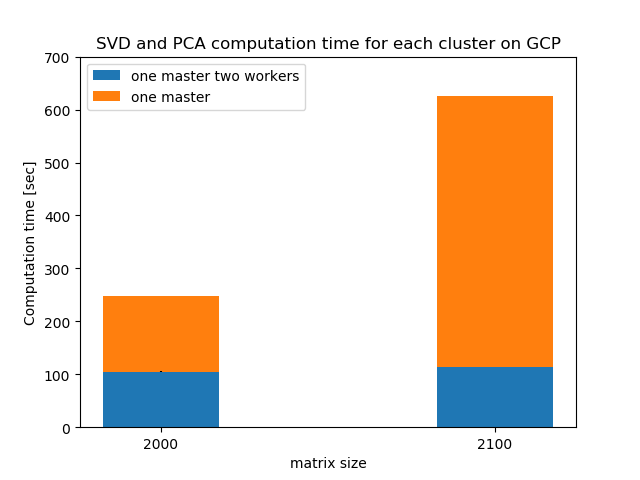
\includegraphics{Figure_1.png}
\caption{SVD and PCA computation for each cluster on GCP}
\label{fig:figure_1}
\end{figure}

Table \ref{tab:table_1} and Figure \ref{fig:figure_1} illustrate that the cluster with high number of
workers outperforms that with low number of workers in terms of
computation time when we increase the matrix size gradually. Also, if
the matrix size is not high enough, then the compuation time between
these clusters can be comparable. In addition, we can see the sub-linear
speedup and faster-than-linear speedup when the benchmarking matrices
with size \(2000\times 2000\) and \(2100\times 2100\) are used from Figure \ref{fig:animals}. Here,
the relative speedup of the algorithm on \(p\) processors is defined as
\(S(p) = t_1/t_p\) , where \(t_1\) and \(t_p\) are the time it takes to
finish the compuations on \(1\) and \(p\) processing units,
respectively.



\iffalse
\begin{longtable}[]{@{}cc@{}}
\toprule
\(2000\times 2000\) & \(2100\times2100\)\tabularnewline
\midrule
\endhead
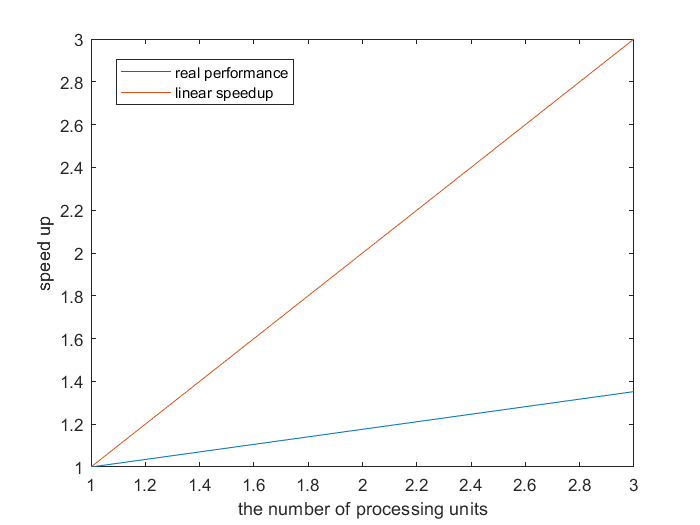
\includegraphics{Figure_speedup_2000.png} &
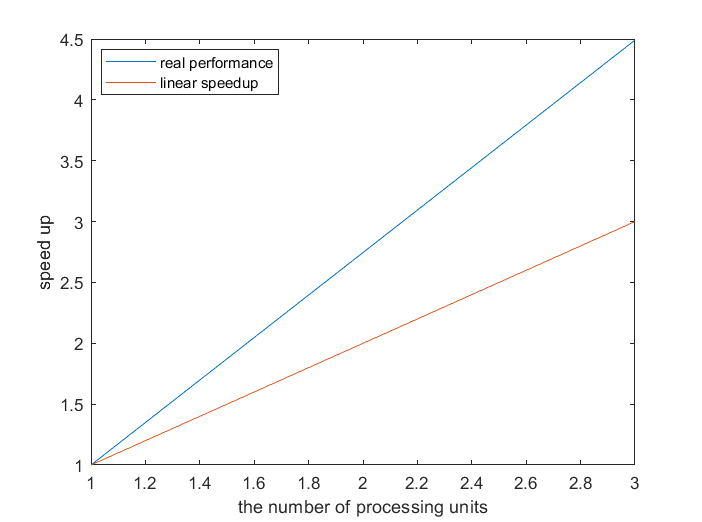
\includegraphics{Figure_speedup_2100.png}\tabularnewline
\bottomrule
\end{longtable}
\fi

\begin{figure}
    \centering
    \begin{subfigure}[b]{0.4\textwidth}
        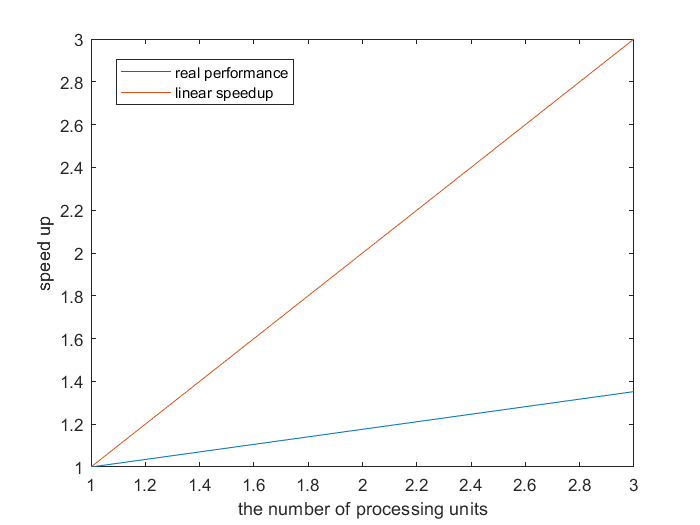
\includegraphics[width=\textwidth]{Figure_speedup_2000.png}
        \caption{$2000\times2000$}
        \label{fig:gull}
    \end{subfigure}
    ~ %add desired spacing between images, e. g. ~, \quad, \qquad, \hfill etc. 
      %(or a blank line to force the subfigure onto a new line)
    \begin{subfigure}[b]{0.4\textwidth}
        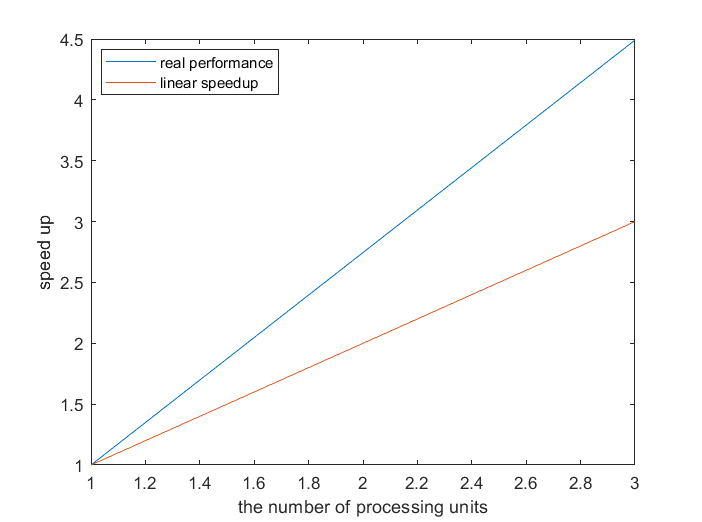
\includegraphics[width=\textwidth]{Figure_speedup_2100.png}
        \caption{$2100\times 2100$}
        \label{fig:tiger}
    \end{subfigure}
    \caption{Speedup for different matrix size}\label{fig:animals}
\end{figure}


\subsection{Reflections}

This assignment enables us to explore how to deploy the codes utilizing the computer clusters on available cloud platforms, e.g. google and amazon clouds. It helps us see the better performance of current parallelism frameworks available in many programming languages to handle computations over large-scale data. 

One complaint would be the installations of \texttt{pyspark} are quite tricky since they require many software packages. However, it is quite convenient to deploy on the google cloud platform using \texttt{dataprocs} which enables us to get the clusters with already installed packages. 

\hypertarget{github-respository}{%
\subsection{Github respository}\label{github-respository}}

All the results and python scripts can be found in the following link:

\url{https://github.com/KhiriratSarit/-Assignment3--Spark-on-gcp}.

\end{document}
